% to compile:
% bibtex proposal
% bibtex proposal
% pdflatex proposal

\documentclass[11pt]{article}   	% use "amsart" instead of "article" for AMSLaTeX format
\usepackage{graphicx}				% Use pdf, png, jpg, or eps§ with pdflatex; use eps in DVI mode
								% TeX will automatically convert eps --> pdf in pdflatex		
\usepackage{amssymb}
\usepackage{hyperref}
\usepackage{graphicx}
\graphicspath{ {./images/} }

\title{Project Proposal: A Domain-Specific Knowledge Graph for News Item Recommendations and Information Retrieval}
\author{Chris Eaves-Kohlbrenner}

\begin{document}
\maketitle

TODO: Cover Page details?

\newpage
\begin{abstract}
This proposal introduces the project plan for a knowledge graph in the news domain. The project is intended to to build a news knowledge graph to enhance recommendations, link prediction, and information retrieval using semantic technologies, natural language processing, and machine learning.

Two phases are planned: (1) build a prototype of a news knowledge graph using a Reuters archive of 59,542 news items and (2) run experiments aimed at enhancing the knowledge graph to improve recommendation quality and information retrieval. Final outcomes will include a functional graph database application and an evaluation documenting any improvements from the experiments.
\end{abstract}

\newpage
\tableofcontents

\newpage
\section{Introduction}
The field of knowledge graphs has seen rapid growth in the last decade, with notable examples like Wikidata, DBpedia, and the Google Knowledge Graph[1]. Meanwhile, the media industry generates a high volume of news content that is often unstructured and semantically limited, presenting information retrieval challenges for news consumers and journalists. The data challenges facing news agencies present an opportunity for a domain-specific knowledge graph architecture. 

Modeling news items as a knowledge graph requires transforming unstructured text or semi-structured XML into a structured and semantically modelled graph structure, which represents meaning or knowledge in the form of graph nodes and edges. The architecture and storage of knowledge graphs can vary, primarily between RDF stores of subject-predicate-object triples and graph databases like Neo4j\cite{zhao2018architecture}. In either case, this graph structure presents opportunities to enrich the data by creating additional edges or relationships between the various entity nodes.

An effective knowledge graph in the news domain would present benefits similar to Wikidata and others: a machine-readable graph enables others to link data and enrich other data sets; journalists can more easily draw insights about the entities in a story; consumers of the news can retrieve more relevant information and recommendations.

\newpage
\section{Literature Review}
\label{sec:LiteratureReview}

A variety of news-specific knowledge systems have been proposed or built to aggregate, generate, and link news data. The efforts described below represent the state of the art for applying knowledge graphs, semantic technology, and natural language processing in the news domain. They form the inspiration for some of the project's architecture and expirementation.

\begin{itemize}
\item \textbf{Neptuno} \cite{castells2004neptuno}, 2004: ``introduction of the emergent semantic-based technologies to improve the processes of creation, maintenance, and exploitation of the digital archive of a newspaper"
\item \textbf{News Engine Web Services (NEWS)} \cite{fernandez2010news}, 2010
\item \textbf{Global Database of Events, Language, and Tone (GDELT)}\footnote{\url{https://www.gdeltproject.org/}}, 2013: graph of news items and events with real-time monitoring of world's news media
\item \textbf{Event Registry} \cite{leban2014event}, 2014: ``a system that can analyse news articles and identify in them mentioned world events"
\item \textbf{NewsReader} \cite{vossen2016newsreader}, 2016: system to read news articles and represent information as RDF; "a cycle of knowledge acquisition and NLP improvement on a massive scale"
\item \textbf{NewsAPI}\footnote{\url{https://newsapi.org/}}, 2017: 
\item \textbf{Reuters' Tracer} \cite{liu2017reuters}, 2017 : ``a system that automates end-to-end news production using Twitter data."
\item \textbf{Scalable Understanding of Multilingual MediA (SUMMA)} \cite{germann2018integrating}, 2018: architecture for monitoring media and applying NLP pipeline
\item \textbf{Acquisition de Schémas pour la Reconnaissance et l'Annotation d'Événements Liés (ASRAEL)} \cite{rudnik2019searching}, 2019: harvest news text, link to Wikidata, and annotate using IPTC rNews vocabulary
\item \textbf{News Graph} \cite{liu2019news}, 2019
\item \textbf{News Hunter} \cite{berven2020knowledge}, 2020
\end{itemize}

The full literature review exercise for the project (\hyperref[sec:PropLiteratureReview]{see Project Plan \#2}) will analyse the news-specific research above, with a specific focus on which ones research knowledge graphs, NLP, statistical ML, and otherwise. This will in turn inform an action plan for the project's knowledge graph architecture and NLP experiments.

In addition to the literature on news-specific knowledge systems, there is a wealth of resources related to knowledge graph architecture more broadly. The project's literature review will also survey and summarise best practices for knowledge graph architecture:

\begin{itemize}
\item Architecture of knowledge graph construction techniques \cite{zhao2018architecture}
\item A review of relational machine learning for knowledge graphs \cite{nickel2015review}
\item Knowledge graph embedding: A survey of approaches and applications \cite{wang2017knowledge}
\item Knowledge Vault: A Web-Scale Approach to Probabilistic Knowledge Fusion \cite{45634}
\end{itemize}

\newpage
\section{Problem Statement and Research Questions}

This project will build a domain-specific knowledge graph of news items. It will use the knowledge graph to prototype a recommendation system and run experiments to improve recommendations and information retrieval.

The planned experiments include:

\begin{itemize}
\item Apply \textbf{semantic technologies (ST)} including ontologies, vocabulary, and RDF
\item Apply \textbf{natural language processing (NLP)} techniques including named entity recognition (NER), clustering and similarity, and keyword extraction for topics, key terms, and locations
\item Apply \textbf{machine learning (ML)} models, including clustering, similarity, and link prediction
\end{itemize}

The key research question for the initial prototype is: \textbf{Can we build a NewsML to Knowledge Graph pipeline, resulting in a knowledge graph that improves news item recommendations and information retrieval?} This pipeline will transform XML/NewsML documents into a knowledge graph, performing ST, NLP, and ML experiments along the way.

Once the KG prototype is in place, the ST, NLP, and ML experiments can be run to enhance the KG. These experiments will investigate some of the following questions:
\begin{itemize}
\item [ST] Can we enhance the data and knowledge graph with semantic technologies, by authoring or integrating with existing OWL ontologies and RDF linked data?
\item [ST] Can we identify which news item relations are relevant for news? Can we remove irrelevant relations?
\item [ST] Can we determine a meaningful level of connection between news items? For example, one-hop, paths of length N, shared entity with salience above some weight/cutoff.
\item [NLP] Can we enhance the data and knowledge graph with named entity recognition?
\item [NLP/ML] Can we extract latent topics, keywords, and locations from news items, as a \textit{category classification} and/or \textit{latent semantic indexing} task?\footnote{Note to self: see NLP week 10 lecture}
\item [NLP/ML] can we identify meaningful clusters of news items?
\item [ML] Can we do link prediction to generate new relationships between news items and entities?\footnote{Project will consider 2.2 example of Donald Trump and Lebron James\cite{liu2019news}}
\item [ML] Can we learn Knowledge Graph Embeddings (KGEs), with the intent to "embed components of a KG including entities and relations into continuous vector spaces, so as to simplify the manipulation while preserving the inherent structure of the KG"?\cite{wang2017knowledge}
\item [ML] In addition to the NLP text extraction methods above, can we use probabilistic methods\cite{45634} or Statistical Relational Learning (SRL)\cite{nickel2015review} to build knowledge graph relationships?
\item [evaluation] How can we evaluate improvements in quality or information retrieval? Which metrics are most meaningful among precision, recall, f-score, and similar?\footnote{
\url{https://en.wikipedia.org/wiki/Evaluation_measures_(information_retrieval)}}
\item [evaluation] Does the knowledge graph improve information retrieval in terms of precision and recall?
\item [evaluation] Does the knowledge graph improve the quality of recommended news items?
\item [evaluation] Can we expose the knowledge graph as a user-facing application, via Neo4j, a user interface, or API?
\item [evaluation] Does the knowledge graph improve human explainability of news item recommendations?
\end{itemize}

\newpage
\section{Proposed Project}
\subsection{Project Technology and Architecture}
The overall project is intended to (1) build a knowledge graph prototype and (2) run NLP experiments to enhance the knowledge graph's news item recommendations and information retrieval. To that end, the project will rely heavily on the following technologies:
\begin{enumerate}
\item Neo4j and Cypher query language
\item Python + Neo4j Python driver
\item OWL / RDF / WikiData / Wikifier
\item NLP...sklearn?
\end{enumerate}

The overall architecture will be structured as a data pipeline with a graph query interface:

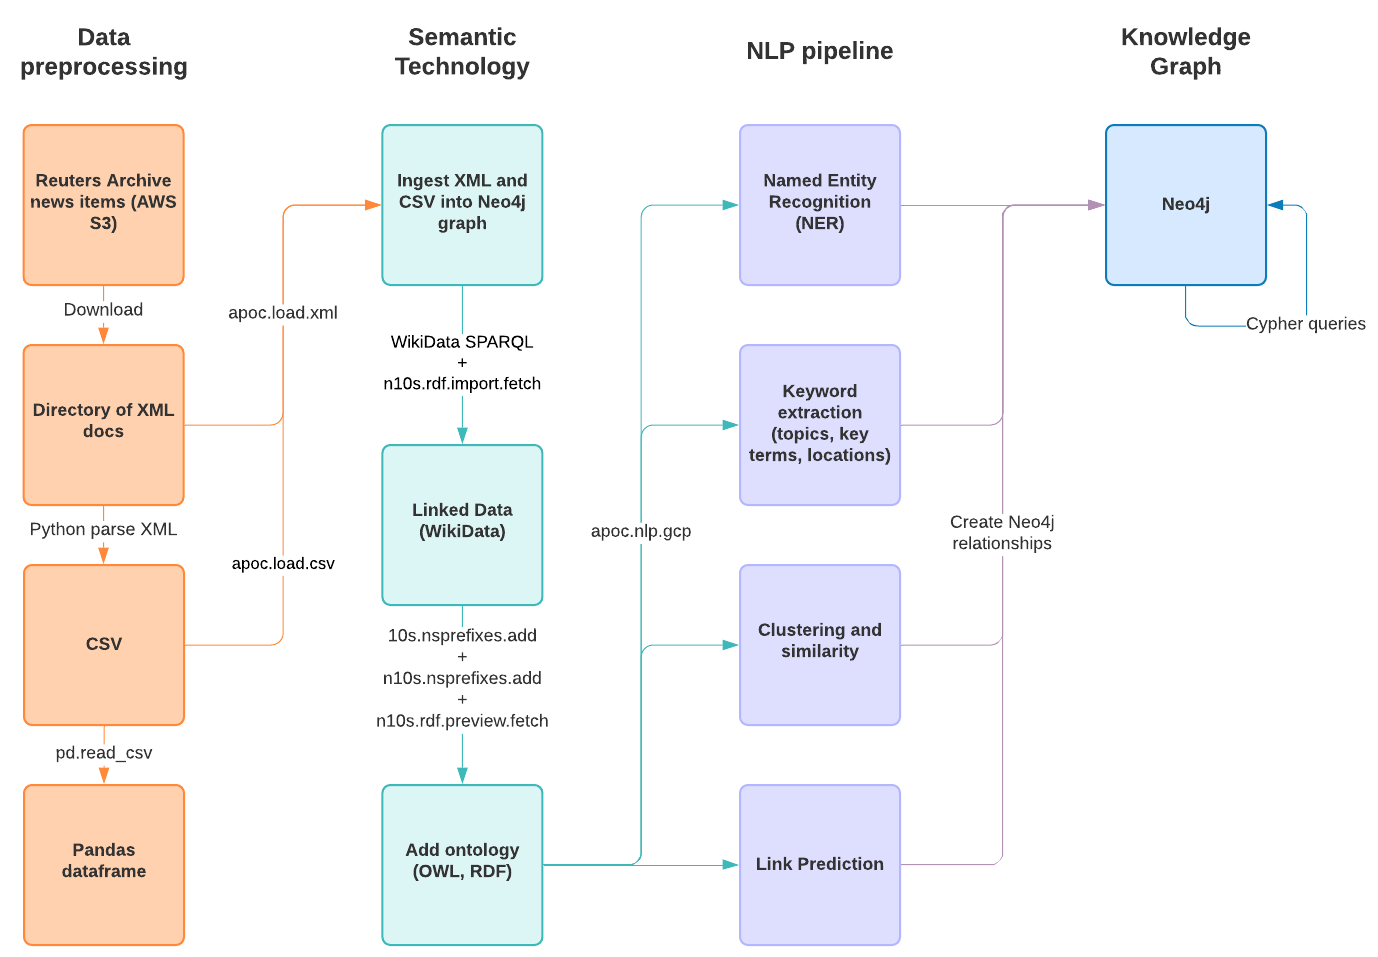
\includegraphics[scale=0.3]{data-pipeline}

The Neo4j interface enables Cypher queries of nodes and relationships.

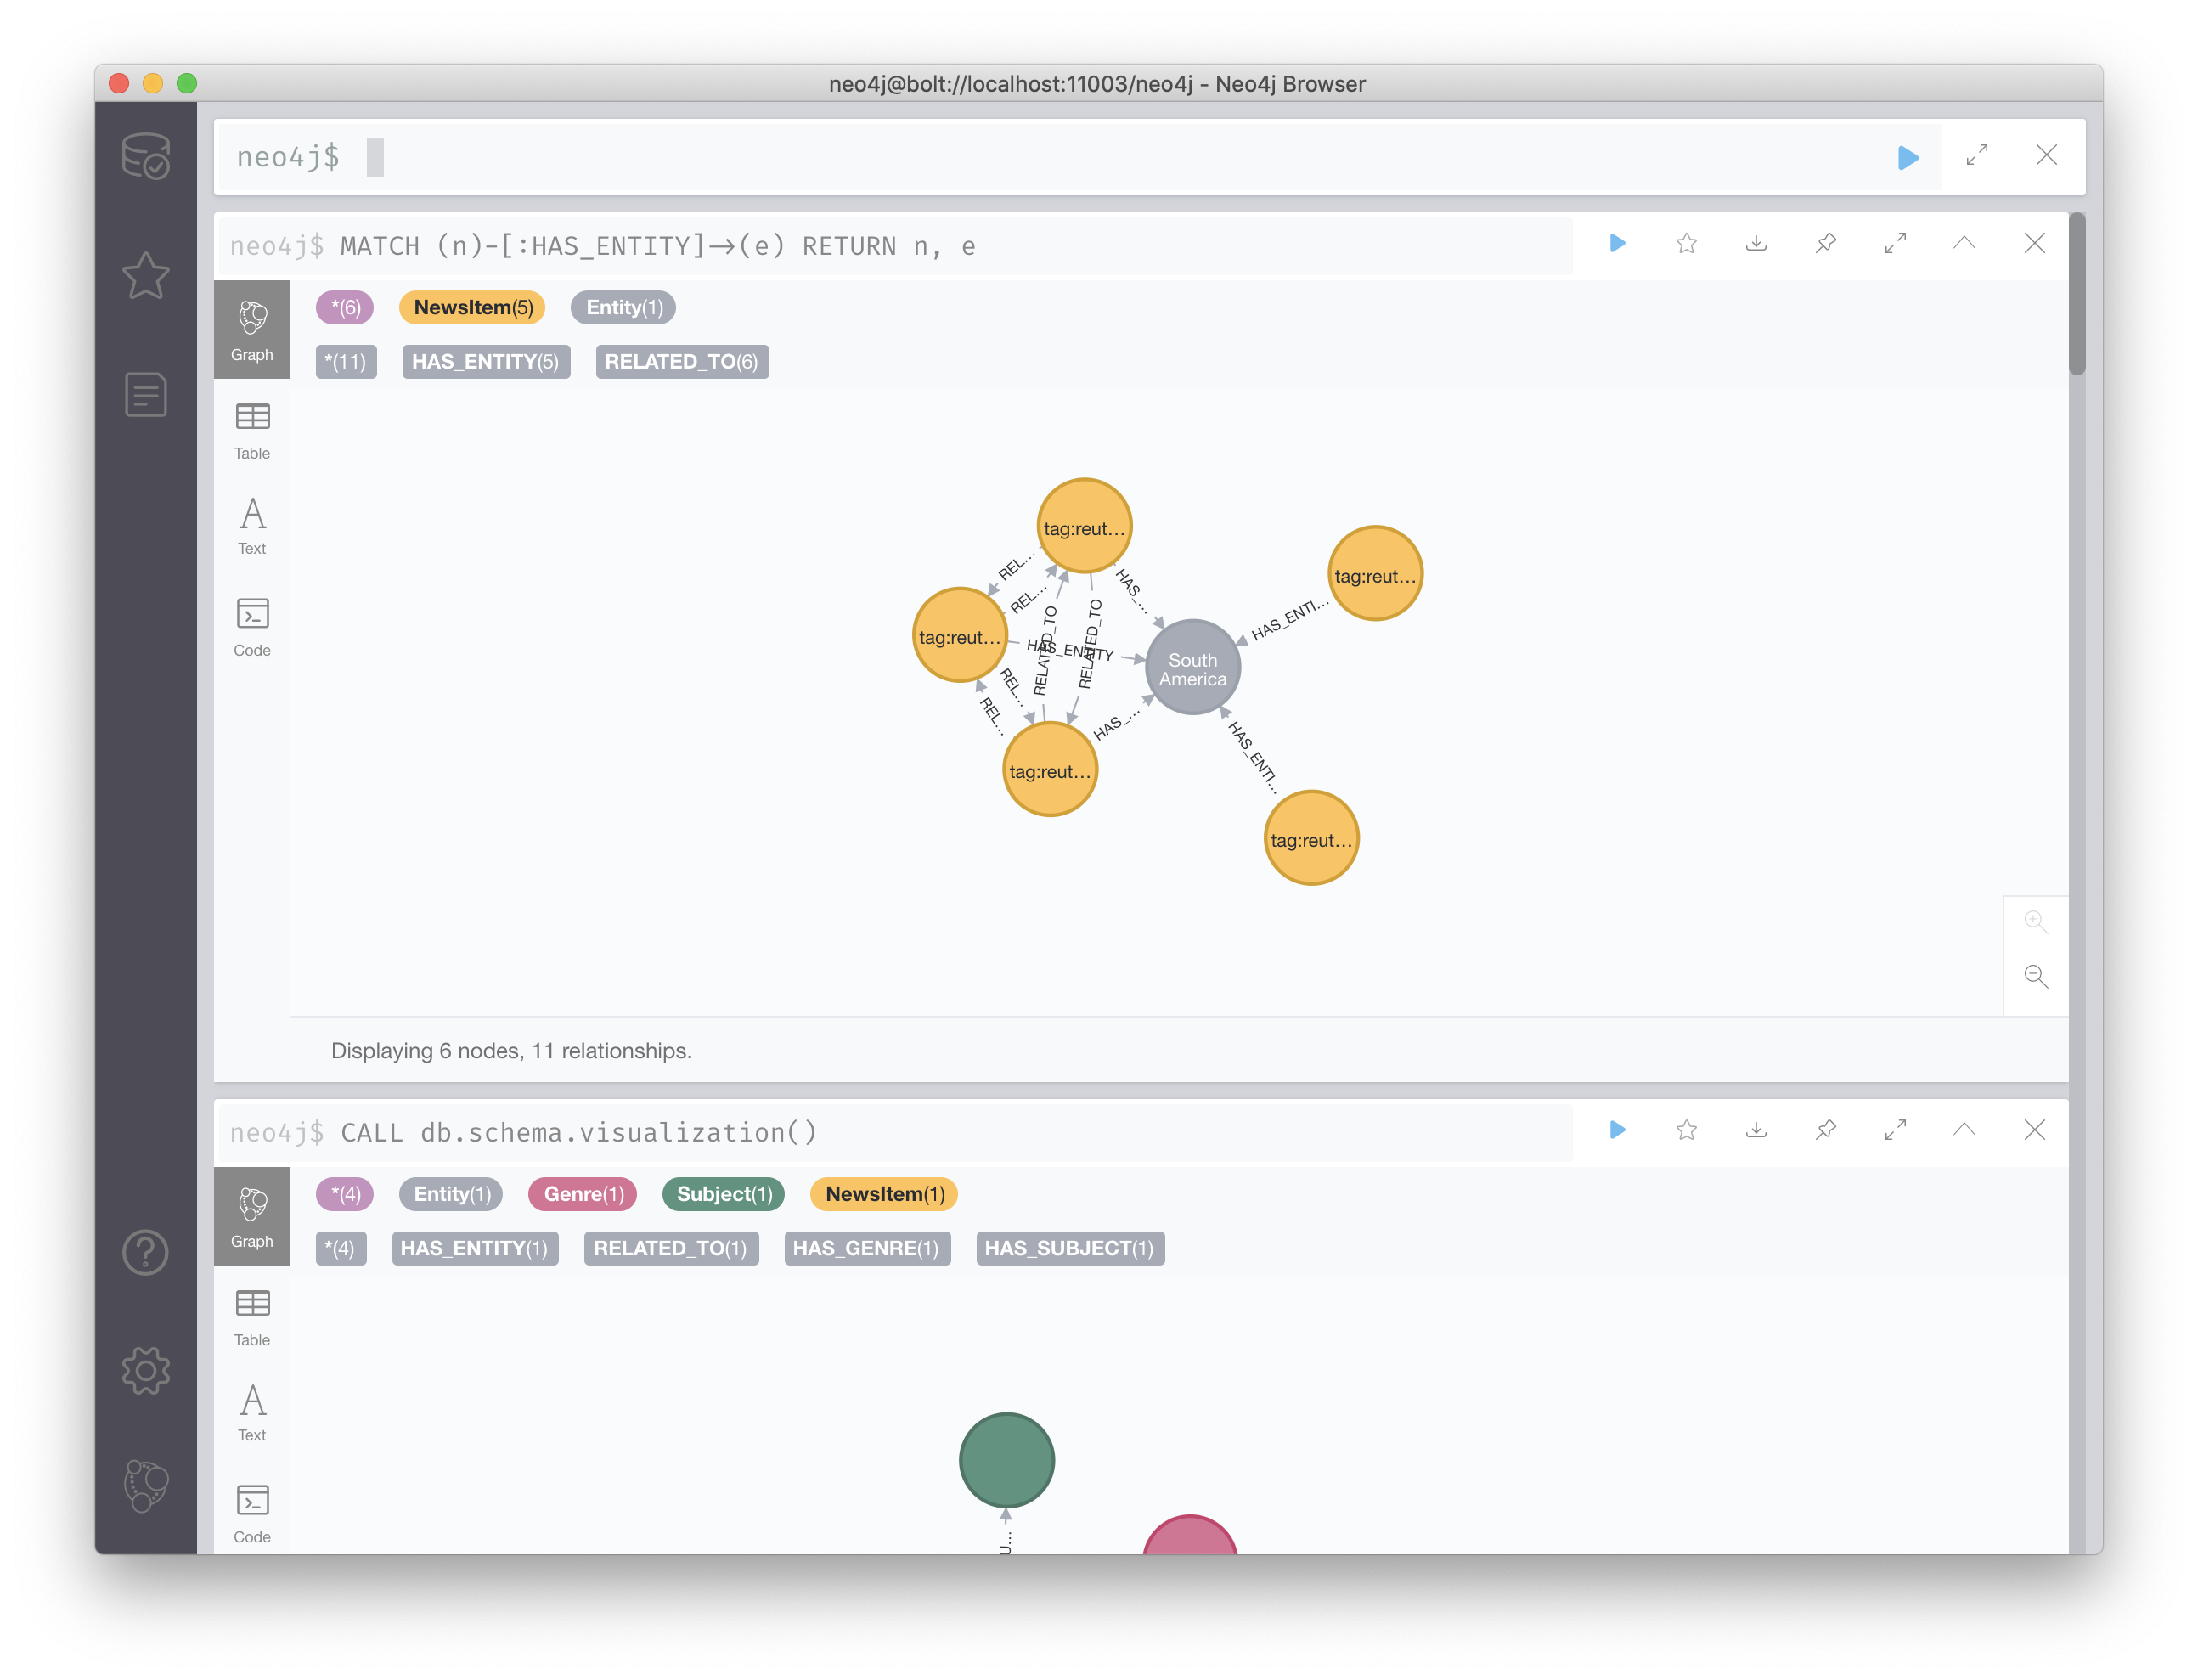
\includegraphics[scale=0.3]{neo4j-cypher-interface}

The end result is an interface by which we can query, for example, all news items that contain a certain entity:

\begin{verbatim}
MATCH (n)-[:HAS_ENTITY]->(e{name:"South America"}) RETURN n, e
\end{verbatim}

Or all items that are related to each other:

\begin{verbatim}
MATCH (n1)-[r:RELATED_TO]->(n2) RETURN n1, r, n2
\end{verbatim}




\subsection{Project Plan}
The project plan is broken into distinct sequential steps:
\begin{enumerate}
\item{Data exploration} \label{sec:PropDataExploration}
  \begin{enumerate}
  \item Clean and analyse dataset of 59,542 Reuters news items\footnote{Sourced from AWS:\\ \url{https://aws.amazon.com/marketplace/pp/Reuters-News-Archive-30-Days/prodview-qwmkdffmmjesa}}
  \item Review structure of news items, including review of NewsML format and intial parsing of XML and text
  \end{enumerate}
\item{Literature Review} \label{sec:PropLiteratureReview}
  \begin{enumerate}
  \item Detailed review of knowledge graph, recommendation and NLP literature (\hyperref[sec:LiteratureReview]{See "Literature Review" above})
  \item Identify architecture, techniques, and analyses from literature to be reused in project knowledge graph and experiments
  \end{enumerate}
\item{Data preprocessing and ingestion} \label{sec:PropDataProcessing}
  \begin{enumerate}
  \item Parse Reuters XML docs to produce dataframe\footnote{Proof of concept completed:\\ \url{https://github.com/heychrisek/msc-data-science-project/blob/main/scripts/item_xml_docs_to_csv.py}}
  \item Ingest subset of Reuters dataset into Neo4j\footnote{Proof of concept in progress:\\ \url{https://github.com/heychrisek/msc-data-science-project/blob/main/scripts/csvs_to_neo4j.cypher}}\footnote{https://neo4j.com/labs/apoc/4.1/import/xml/}
  \end{enumerate}
\item{Graph modeling and ST experiments} \label{sec:PropGraphModeling}
  \begin{enumerate}
  \item Build Neo4j/Cypher queries for similar content (e.g., item that’s no more than X steps away via topic or items within date range)
  \item Use Neo4j, APOC, and neosemantics to link Wikidata\footnote{\url{https://neo4j.com/developer/graph-data-science/build-knowledge-graph-nlp-ontologies/}}\footnote{Wikidata script in progress:\\ \url{https://github.com/heychrisek/msc-data-science-project/blob/main/scripts/wikidata_to_wikipedia_url.py}}
  \item Use Neo4j, APOC, and neosemantics to integrate ontology\footnote{\url{https://neo4j.com/developer/graph-data-science/build-knowledge-graph-nlp-ontologies/} and attempt ST experiments to build ontology and link data}
  \item Define graph model\footnote{https://neo4j.com/developer/guide-data-modeling/}. Initial proof of concept graph model:\\ 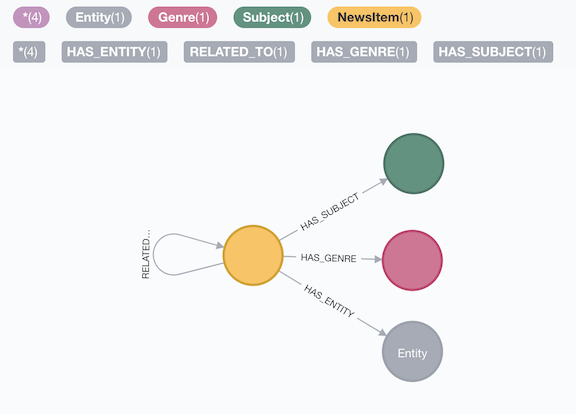
\includegraphics{graph-model}
  \item Complete Knowledge Graph prototype
  \end{enumerate}
\item{Enhance knowledge graph with NLP experiments} \label{sec:PropNLP}
  \begin{enumerate}
  \item NLP models for similarity\footnote{TF-IDF: \url{https://towardsdatascience.com/the-best-document-similarity-algorithm-in-2020-a-beginners-guide-a01b9ef8cf05}}, clustering, keywords, and topics
  \item Language models to predict what a story is about
  \footnote{Resources: \url{http://www.mmds.org} (chapter 3) \\ \url{https://www.youtube.com/watch?v=c6xK9WgRFhI}}
  \item Evaluate NLP experiment
  \item Generate Neo4j knowledge graph relationships between similar items
  \end{enumerate}
\item{[OPTIONAL] Additional considerations if time allows} \label{sec:PropOptional}
  \begin{enumerate}
  \item ML experimentation: probabilistic links and statistical relational learning\cite{nickel2015review}
  \item Prepare a production-ready Neo4j demo, including cloud hosting
  \footnote{\url{https://neo4j.com/developer/guide-cloud-deployment/} \\ \url{https://aws.amazon.com/marketplace/pp/B071P26C9D} \\ \url{https://neo4j.com/developer/neo4j-cloud-aws-ec2-ami/} }
  \item Expose public Cypher query interface/API
  \item Expose web user interface
  \item Build chatbot interface
  \end{enumerate}
\item Finalise written report \label{sec:PropWrittenReport}
  \begin{enumerate}
  \item Evaluate knowledge graph recommendations
  \item Evaluate results of NLP experiments
  \item Evaluate final architecture relative to diagrams below
  \end{enumerate}
\end{enumerate}


\subsection{Risks and Mitigation}
\begin{enumerate}
\item Risk: Unrealistic scope \\
Impact: failure to deliver all aspects of project plan \\
Mitigation: identify “must-have”/“MVP”
\item Risk: Personal circumstances around child's birth in May \\
Impact: may not strictly follow project timeline \\
Mitigation: follow Kanban, not waterfall
\item Risk: Limited success of NLP techniques \\
Impact: failure to generate meaningful recommendations; failure to improve precision/recall \\
Mitigation: can still learn from experimentation (learn what doesn’t work)
\item Risk: Failed integration with certain technologies (Samtla, etc.) \\
Impact: failure to use one tech \\
Mitigation: can use other tech
\item Risk: Challenges to AWS hosting (cost, scale) \\
Impact: failure to publicly expose/demo the graph database \\
Mitigation: provide local Neo4j/API demo
\end{enumerate}


\subsection{Project timeline}
The following breaks down the approximate intended deliverable by each week.

\begin{itemize}
\item [\textbf{Week}] \textbf{Deliverable}
\item [April 11] Project proposal submission
\item [April 18] Complete initial data exploration/analysis (\hyperref[sec:PropDataExploration]{Project Plan \#1})
\item [April 25] Complete literature review (\hyperref[sec:PropLiteratureReview]{\#2})

\item [May 2]
\item [May 9] Complete initial preprocessing and Neo4j ingestion
\item [May 16] Provide sample Cypher queries
\item [May 23] Complete data processing and ingest (\hyperref[sec:PropDataProcessing]{\#3})
\item [May 30]

\item [June 6]
\item [June 13] Begin graph modeling (\hyperref[sec:PropGraphModeling]{\#4})
\item [June 20]
\item [June 27] Complete knowledge graph prototype (\hyperref[sec:PropGraphModeling]{\#4})

\item [July 4] Begin NLP experiment (\hyperref[sec:PropNLP]{\#5})
\item [July 11]
\item [July 18]
\item [July 25] Complete NLP experiments (\hyperref[sec:PropNLP]{\#5})

\item [August 1] Evaluation of NLP experiments, information retrieval, and recommendations
\item [August 8]
\item [August 15]
\item [August 22]
\item [August 29] Report writing ((\hyperref[sec:PropWrittenReport]{\#7}))

\item [September 5]
\item [September 12]
\item [September 16] Project submission
\end{itemize}

\newpage
\section{Conclusion}
\subsection{Targeted Outcomes}

As mentioned above, the key research question is \textbf{can we build a NewsML to Knowledge Graph pipeline, resulting in a knowledge graph that improves news item recommendations and information retrieval?} Therefore the desired outcome is an affirmative answer to this question. Furthermore, outcome will include a summary of NLP techniques applied to the knowledge graph and an evaluation of how they have succeeded. Finally, the enhanced knowledge graph will be made available to demo sample queries, recommendations, and information retrieval.

\subsection{Personal Comments}

This proposal concludes with a few personal comments regarding the project motivation and desired personal outcomes. As a member of the product engineering team at Reuters, the author hopes to (1) understand the news industry, data, and knowledge representation efforts at a deeper level; (2) apply an understanding of the news industry and Reuters-specific data to generate domain insights; and (3) as a best case scenario, create meaningful value for Reuters and the news broader industry.

This project is the culmination of the MSc Data Science degree and therefore aims to combine key learnings from data science, semantic technology, natural language processing, and information retrieval into a single research and software development project.

\newpage
\section{Glossary}
\begin{itemize}
\item KG - Knowledge Graph
\item ML - Machine Learning
\item NewsML\footnote{\url{https://iptc.org/standards/newsml-g2/}} - XML format for news items and metadata
\item OWL - Web Ontology Language
\item NLP - Natural Language Processing
\item SRL - Statistical Relational Learning
\item ST - Semantic Technology
\item XML - Extensible Markup Language format for encoding documents
\end{itemize}

\newpage
\bibliographystyle{abbrv}
\bibliography{proposal}

\end{document}  